\documentclass[a4paper, 10pt, conference]{IEEEtran}

\usepackage[utf8]{inputenc}
\usepackage[T1]{fontenc}
\usepackage[
	colorlinks=true,
	linkcolor=black,
	anchorcolor=black,
	citecolor=black,
	filecolor=black,
	menucolor=black,
	runcolor=black,
	urlcolor=black
]{hyperref}
\usepackage{url}
\usepackage{graphicx}
\usepackage[ngerman]{babel}
\usepackage[style=ieee]{biblatex}

\addbibresource{references.bib}

\graphicspath{ {./images/} }

\title{\LARGE
\textbf{Reddiment: Reddit Sentiment-Analyse} \\ Technical Report
}

\author{
\IEEEauthorblockN{Tobias Bauer} \IEEEauthorblockA{\textit{t.bauer@oth-aw.de}}\and
\IEEEauthorblockN{Fabian Beer} \IEEEauthorblockA{\textit{f.beer1@oth-aw.de}}\and
\IEEEauthorblockN{Daniel Holl} \IEEEauthorblockA{\textit{d.holl1@oth-aw.de}}\and\and[\\]\and
\IEEEauthorblockN{Ardian Imeraj} \IEEEauthorblockA{\textit{a.imeraj@oth-aw.de}}\and
\IEEEauthorblockN{Konrad Schweiger} \IEEEauthorblockA{\textit{k.schweiger@oth-aw.de}}\and
\IEEEauthorblockN{Philipp Stangl} \IEEEauthorblockA{\textit{p.stangl1@oth-aw.de}}\and
\IEEEauthorblockN{Wolfgang Weigl} \IEEEauthorblockA{\textit{w.weigl@oth-aw.de}}\and
}

\begin{document}

\maketitle
\thispagestyle{empty}
\pagestyle{empty}

\begin{abstract}
Dieser Technical Report beschreibt die Architektur von Reddiment -- ein webbasiertes Dashboard zur Sentiment-Analyse von Subreddits. 
\end{abstract}

\section{Einführung und Ziele}

\texttt{r/wallstreetbets}, auch bekannt als WallStreetBets oder WSB, ist ein Subreddit, in dem über Aktien- und Optionshandel spekuliert wird.  Der Subreddit ist bekannt für seine profane Art und die Vorwürfe, dass Nutzer/innen Wertpapiere manipulieren und volatile Kursbewegungen auslösen.
Anhand von Sentiment-Analyse sollen nun Subreddits in Bezug auf Aktienkursverläufe analysiert werden. Dazu soll ein webbasiertes Dashboard entwickelt werden \dots

In den weiteren Abschnitten des Technical Reports wird zuerst die Bausteinsicht des Gesamtsystems in Abschnitt~\ref{s:bausteinsicht} eingegangen. Im nächsten Abschnitt~\ref{s:verteilungssicht} wird die Verteilungssicht der Anwendung beschrieben. In Abschnitt~\ref{s:entwicklungswerkzeuge} werden die angewandten Werkzeuge zur Entwicklung der Anwendung vorgestellt. Abschließend wird kurz auf die angewandten Sicherheitskonzepte in Abschnitt~\ref{s:sicherheitskonzepte} eingegangen und ein Fazit in Abschnitt~\ref{s:fazit} gegeben, gefolgt vom Literaturverzeichnis am Ende.

\section{Bausteinsicht} \label{s:bausteinsicht}
Diese Sicht zeigt die statische Zerlegung des Systems in Bausteine sowie deren Beziehungen. 

\subsection{Gesamtsystem}
%Whitebox-Beschreibung des Gesamtsystems, zusammen mit Blackbox-Beschreibungen der darin enthaltenen Bausteine.
Reddiment bezieht Daten aus mehreren Quellen und stellt diese dem Benutzer aggregiert bereit. Die folgende Abbildung \ref{fig:context} zeigt die Interaktionen des Systems mit Fremdsystemen und dem Benutzer.

\begin{figure}[ht]
	\centering
	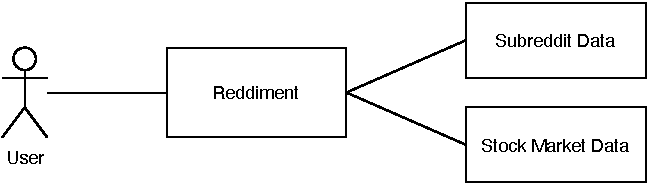
\includegraphics[width=\linewidth]{context}
	\caption{Reddiment Gesamtsystem}
	\label{fig:context}
\end{figure}

\subsection{Backend}
Dieser Abschnitt beschreibt die server-seitige Backend-Architektur.

\subsubsection{Laufzeitumgebung}

JavaScript-basierte Plattform Node.js mit dem serverseitigen Webframework ExpressJS.


\subsection{Datenbank} \label{datenbank}

Die Speicherung der Daten erfolgt mit Elasticsearch.


\subsection{Dienste}
Dieser Abschnitt beschreibt die Dienste (engl. Services).

\subsubsection{Sentiment}

In diesem Dienst \dots

\subsubsection{Reddit Crawler}

Der Reddit Crawler


\subsection{Frontend}
Dieser Abschnitt beschreibt die client-seitige Frontend-Architektur.
Das Frontend wird unter Zuhilfenahme des Frontend-Frameworks SvelteKit realisiert.
Es ist selbst in zwei Unter-Bausteine zerlegt:

\subsubsection{Components}

In diesem Modul sind die Svelte-Komponenten gesammelt, mit denen die eigentliche Anzeige im Webbrowser realisiert wird.
Die Komponenten behandeln alle Eingaben und kommunizieren bei Bedarf mit dem Backend über die GraphQL API Schnittstelle.


\section{Verteilungssicht} \label{s:verteilungssicht}
Das Verteilungssicht beschreibt die Verteilung des Gesamtsystems,  wichtige Begründungen für diese Verteilungsstruktur und die Zuordnung von Softwareartefakten zu Bestandteilen der Infrastruktur.
Zentrale Bestandteile der Verteilungsstruktur sind \dots

\begin{figure*}[ht]
	\centering
	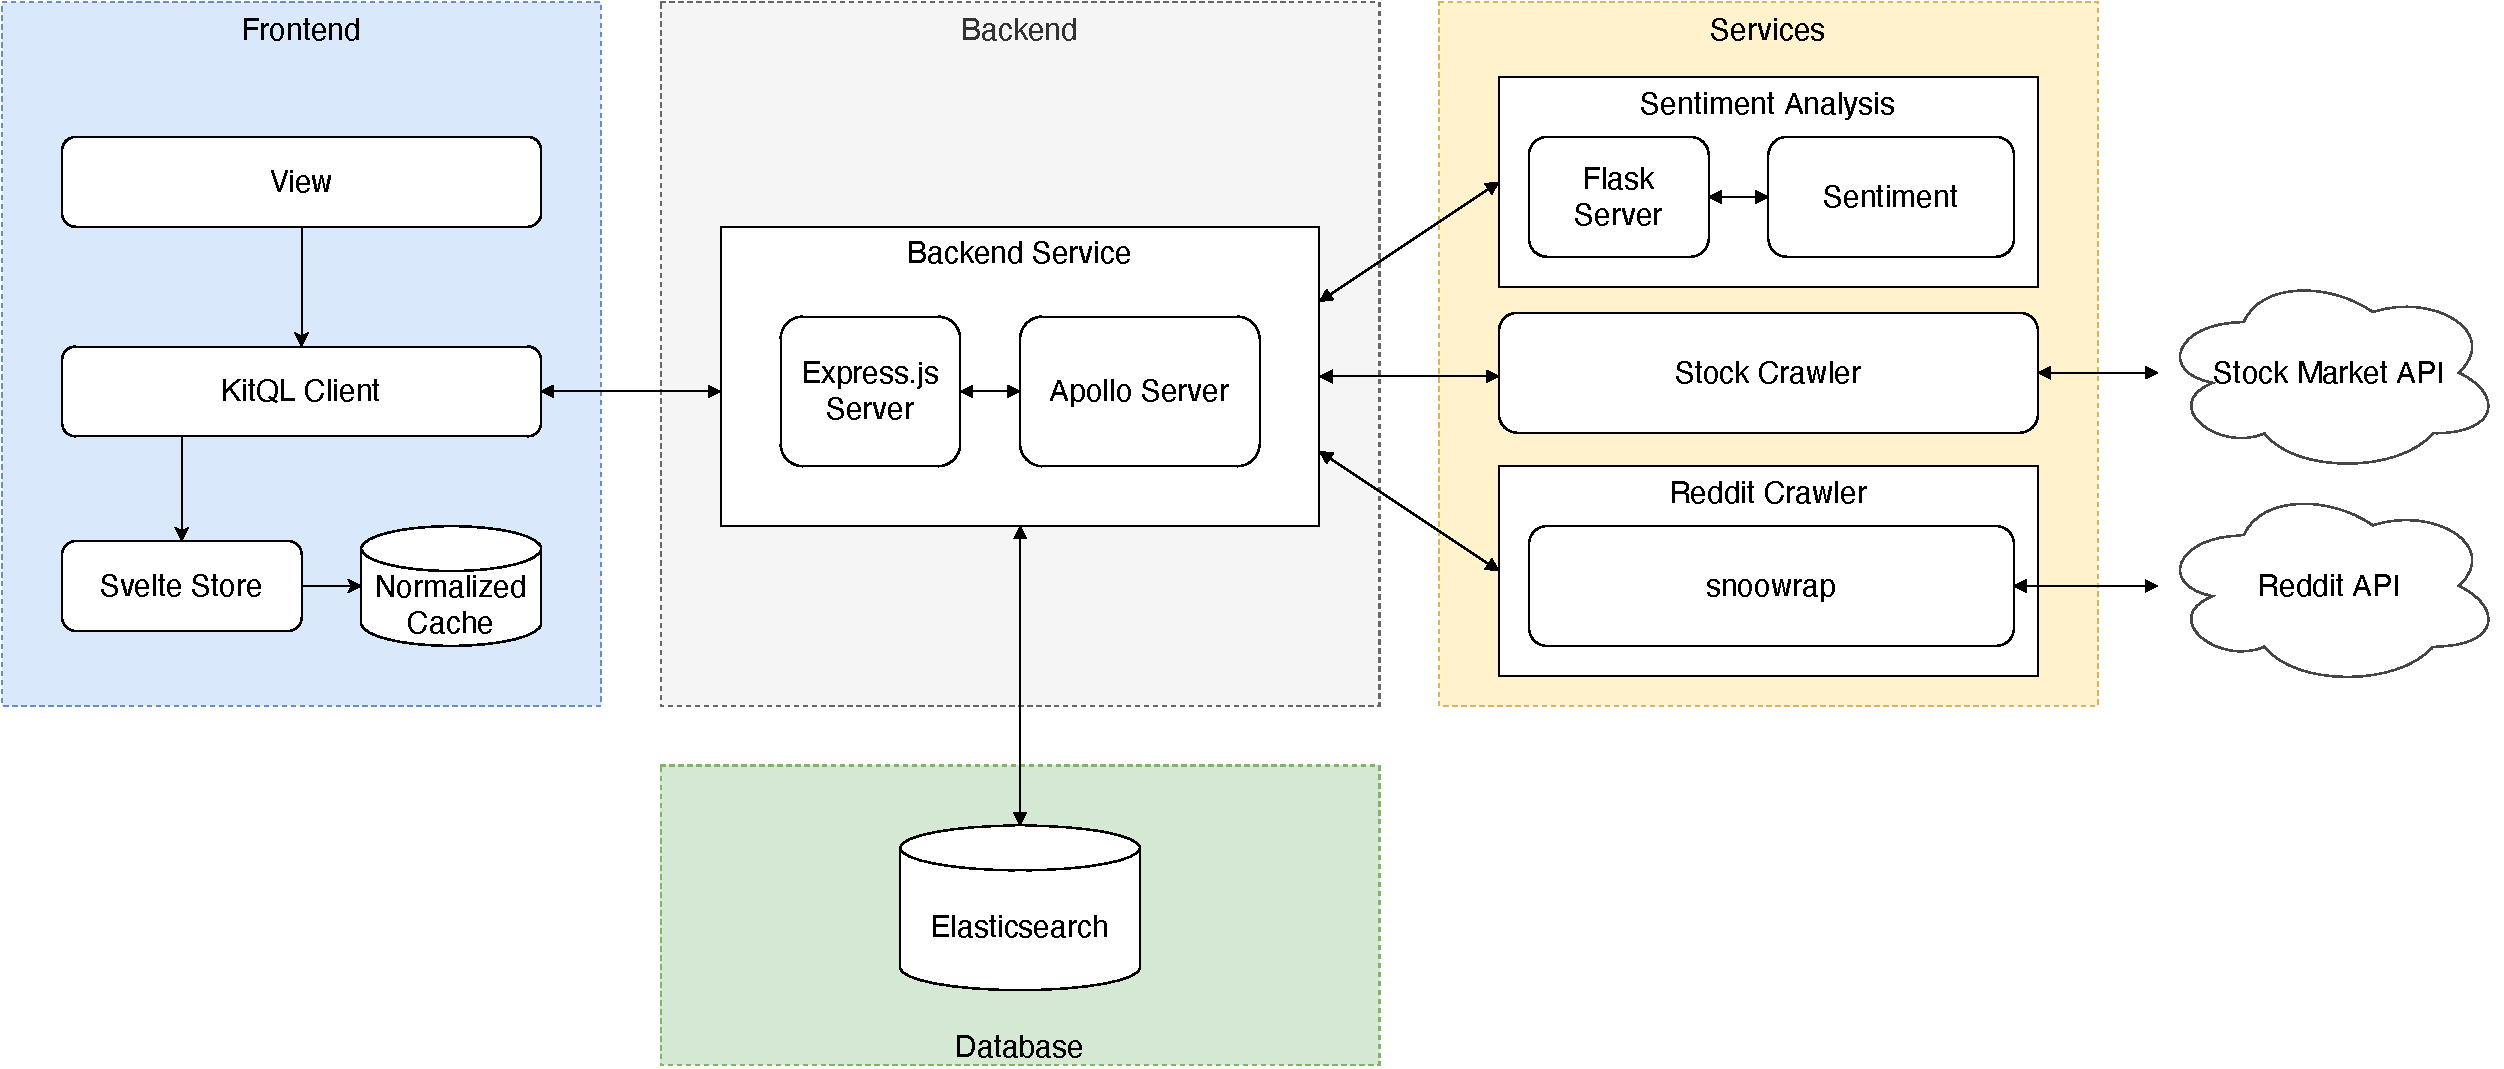
\includegraphics[width=\linewidth]{architecture}
	\caption{Überblick über die Architektur von Reddiment. Die Architektur besteht aus vier Teilen: Das Frontend bietet dem Nutzer eine graphisches Dashboard zur Visualisierung der Metriken (Abschnitt ),  das Backend umfasst (Abschnitt ),  die Datenbank (Abschnitt ) ist ,  und den Diensten (engl. Services) zur Sentiment Analyse als auch zum crawlen der Daten von externen APIs.}
	\label{fig:architecture}
\end{figure*}

Tailwind CSS

\section{Entwicklungswerkzeuge} \label{s:entwicklungswerkzeuge}

Im folgenden Abschnitt wird auf die verwendeten Entwicklungswerkzeuge eingegangen.

\subsection{Paketverwaltung}

Die Verwaltung der Abhängigkeiten erfolgt mit „npm“.

\subsection{Linting}

In beiden Unterprojekten (Frontend und Backend) wird jeweils „eslint“ in Verbindung mit „prettier“ verwendet,
um die Einhaltung der Codierrichtlinien zu gewährleisten.

Die Konfigurationen sind jeweils in den Dateien \texttt{eslintrc.js} und \texttt{prettierrc.js} hinterlegt.

\subsection{Build-Tools}

\subsubsection{Backend}

Im Backend wird der Typescript Compiler „tsc“ verwendet, um die Dateien in ein Format zu überführen,
welches mit \texttt{node} ausgeführt werden kann.

Die Konfiguration findet sich dabei in der Datei \texttt{tsconfig.json}.

\subsubsection{Frontend}
Im Frontend ist Vite dafür zuständig, die Anwendung aus dem Quellcode zu erstellen. Dabei gibt es zwei Varianten:
Für Entwicklungszwecke wird ein Vite-Dev-Server (mit Reload-Funktionalität) zum Bereitstellen der Anwendung verwendet,
während für den Produktiveinsatz nur die benötigten Zieldateien unter Verwendung des \texttt{Static adapter} erstellt werden, die dann mit einer beliebigen Server-Software ausgeliefert werden können. 

Ferner sind Alias-Namen für häufig genutzte Verzeichnisse definiert, um Pfadangaben zu vereinfachen.

\subsection{Unit Tests}

Im Backend werden Unit-Tests anhand von „mocha“ \cite{mochajs} durchgeführt. Außerdem wird „nyc“ \cite{instanbuljs} für die Erzeugung der Test Abdeckung verwendet. 

Im Frontend wird „Vitest“ \cite{vitest} verwendet. Für die Frontend-Komponenten wird zusätzlich die „svelte-testing-library“ \cite{stl} verwendet. Diese ermöglicht es, die Komponenten zu \textit{rendern} und Details über die verschiedenen Elemente innerhalb der Komponente zu erhalten.

\section{Sicherheitskonzepte} \label{s:sicherheitskonzepte}

Dieser Abschnitt beschreibt die angewendeten Sicherheitskonzepte, die für eine sichere Entwicklungs- und Produktionsumgebung notwendig sind.

\subsection{Secrets Verwaltung}

\dots

\section{Fazit und Ausblick} \label{s:fazit}

\dots

\printbibliography

\end{document}

